% RESULTADOS-------------------------------------------------------------------

\chapter{RESULTADOS}
\label{chap:resultados}

%Cada capítulo deve conter uma pequena introdução (tipicamente, um ou dois parágrafos) que deve deixar claro o objetivo e o que será discutido no capítulo, bem como a organização do capítulo. 

Após a formulação e teste de cada item dos sistemas deu-se início a junção de todas as funcionalidades arquitetadas. O conteúdo deste capítulo visa apresentar os resultados obtidos neste trabalho em cada área de desenvolvimento.

Primeiramente como resultado da parte de \textit{hardware} podemos apresentar a formulação dos circuitos dos módulos \textbf{CCM} e \textbf{TCM} apresentados nas figuras abaixo. Os dois módulos foram montados em \textit{protoboard} buscando validar, em conjunto, todas funcionalidades as seções descritas na metodologia.


\begin{figure}[H]
	\centering
	\caption{Protótipo montado.}
	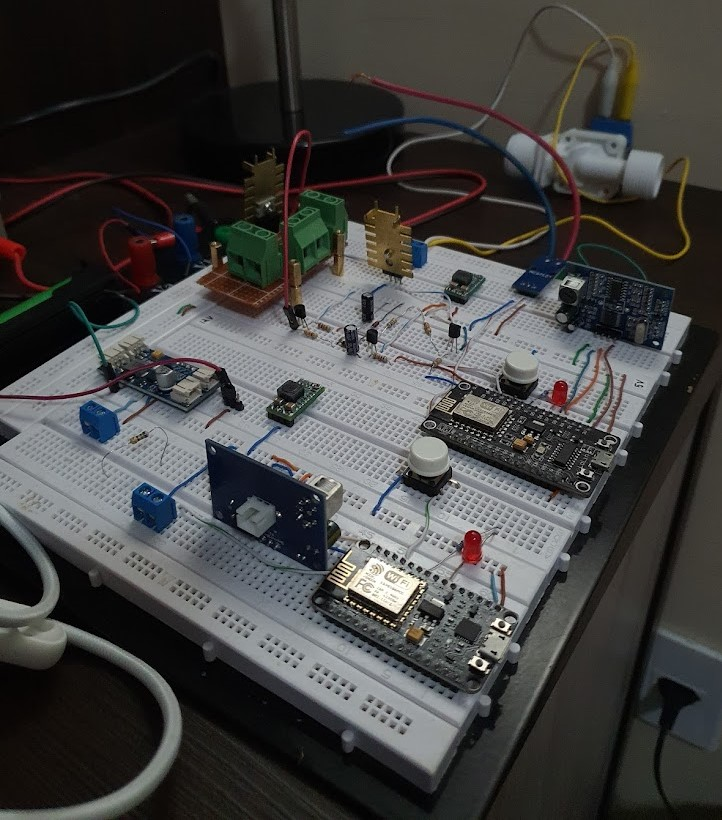
\includegraphics[width=0.6\textwidth]{figuras/esquema_protoboard.jpg}
	\fonte{Própria}
	\label{fig:figma_plan_desktop}
\end{figure}

Também foram desenvolvidos os esquemáticos dos dois módulos (\autoref{fig:kicad_ccm}), levando em consideração todas as ligações: circuitos de alimentação, sensoriamento e comunicação. Esse resultado garante futuras implementações de \textit{layout's 3D} e confecção das placas de circuito impresso.


\begin{figure}[H]
	\centering
	\caption{Esquemático do módulo CCM implementado no Kicad.}
	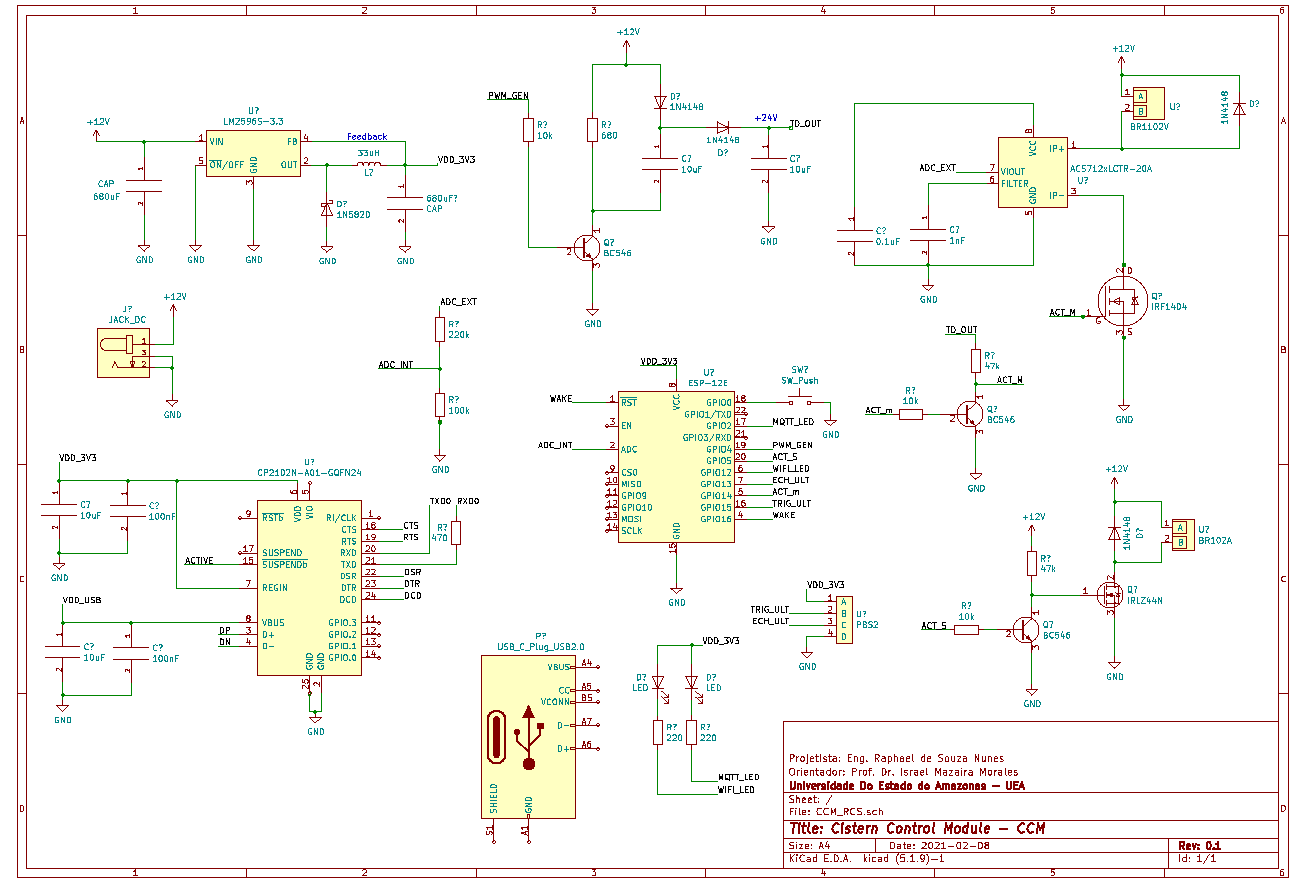
\includegraphics[width=1\textwidth]{figuras/kicad_ccm.png}
	\fonte{Própria}
	\label{fig:kicad_ccm}
\end{figure}



No quesito de \textit{firmware}, alcançou-se todas as funcionalidades propostas, gerando um código estável e escalável para projetos reais. Os códigos associados podem ser acessados no \textit{Github}. O código principal, \autoref{fig:tcm_main}, conta com diversos arquivos de cabeçalho que modularizam as funcionalidades: 

\begin{enumerate}
	\item \textit{Libraries.h}: ficam armazenadas as bibliotecas de terceiros que foram utilizadas;
	\item \textit{GeneralDefinitions.h}: são definidos os pinos e são iniciadas as variáveis globais;
	\item \textit{Interruptions.h}: é implementado a funcionalidade de \textit{Factory Reset} por meio de interrupção externa (botão);
	\item \textit{Sleep\_Functions.h} possui funções de modo de \textit{DeepSleep}, porém este modo não é utilizado;
	\item  \textit{SimpleBlink.h}: define o compotamento dos leds;
	\item \textit{Driver\_ConfigTCM.h} ou \textit{Driver\_ConfigCCM.h} define e manipula os arquivos de configuração do microcontrolador;
	\item \textit{Driver\_RWS.h}: é utilizado para leitura e escrita no sistema de arquivos interno;
	\item \textit{Driver\_WIFI.h}: define as funções de conexão e modos de operação do \textit{chip} de WI-FI;
	\item \textit{Driver\_MQTT.h}: é utilizado para configurar a conexão com o \textit{broker} assim como definir os \textit{callbacks};
	\item \textit{OTA\_upgrade.h}: utiliza os métodos para atualização via \textit{internet};
	
\end{enumerate}

  
\begin{figure}[H]
	\centering
	\caption{Versão final do código do \textit{firmware}}
	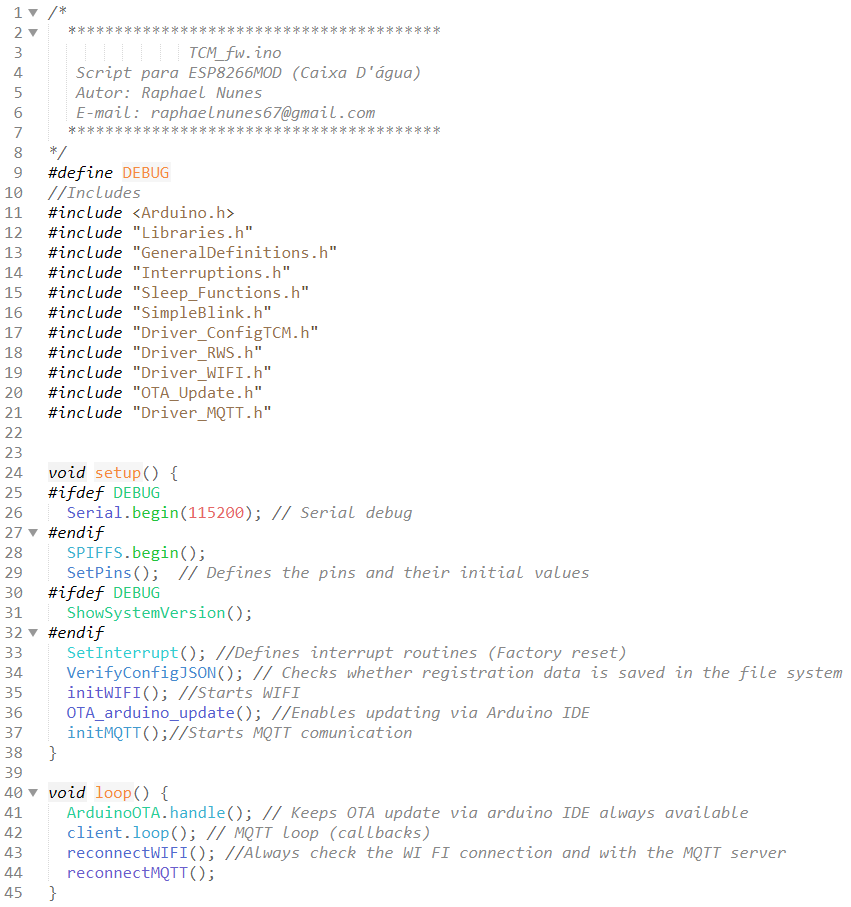
\includegraphics[width=1\textwidth]{figuras/tcm_main.png}
	\fonte{Própria}
	\label{fig:tcm_main}
\end{figure}


Por fim, também obtivemos como resultado a elaboração de telas utilizando as tecnologias propostas, atingindo o objetivo de relacionar o \textit{software} com as camadas de \textit{firmware} e \textit{hardware}. 

\begin{figure}[H]
	\centering
	\caption{Implementação da aplicação \textit{desktop}.}
	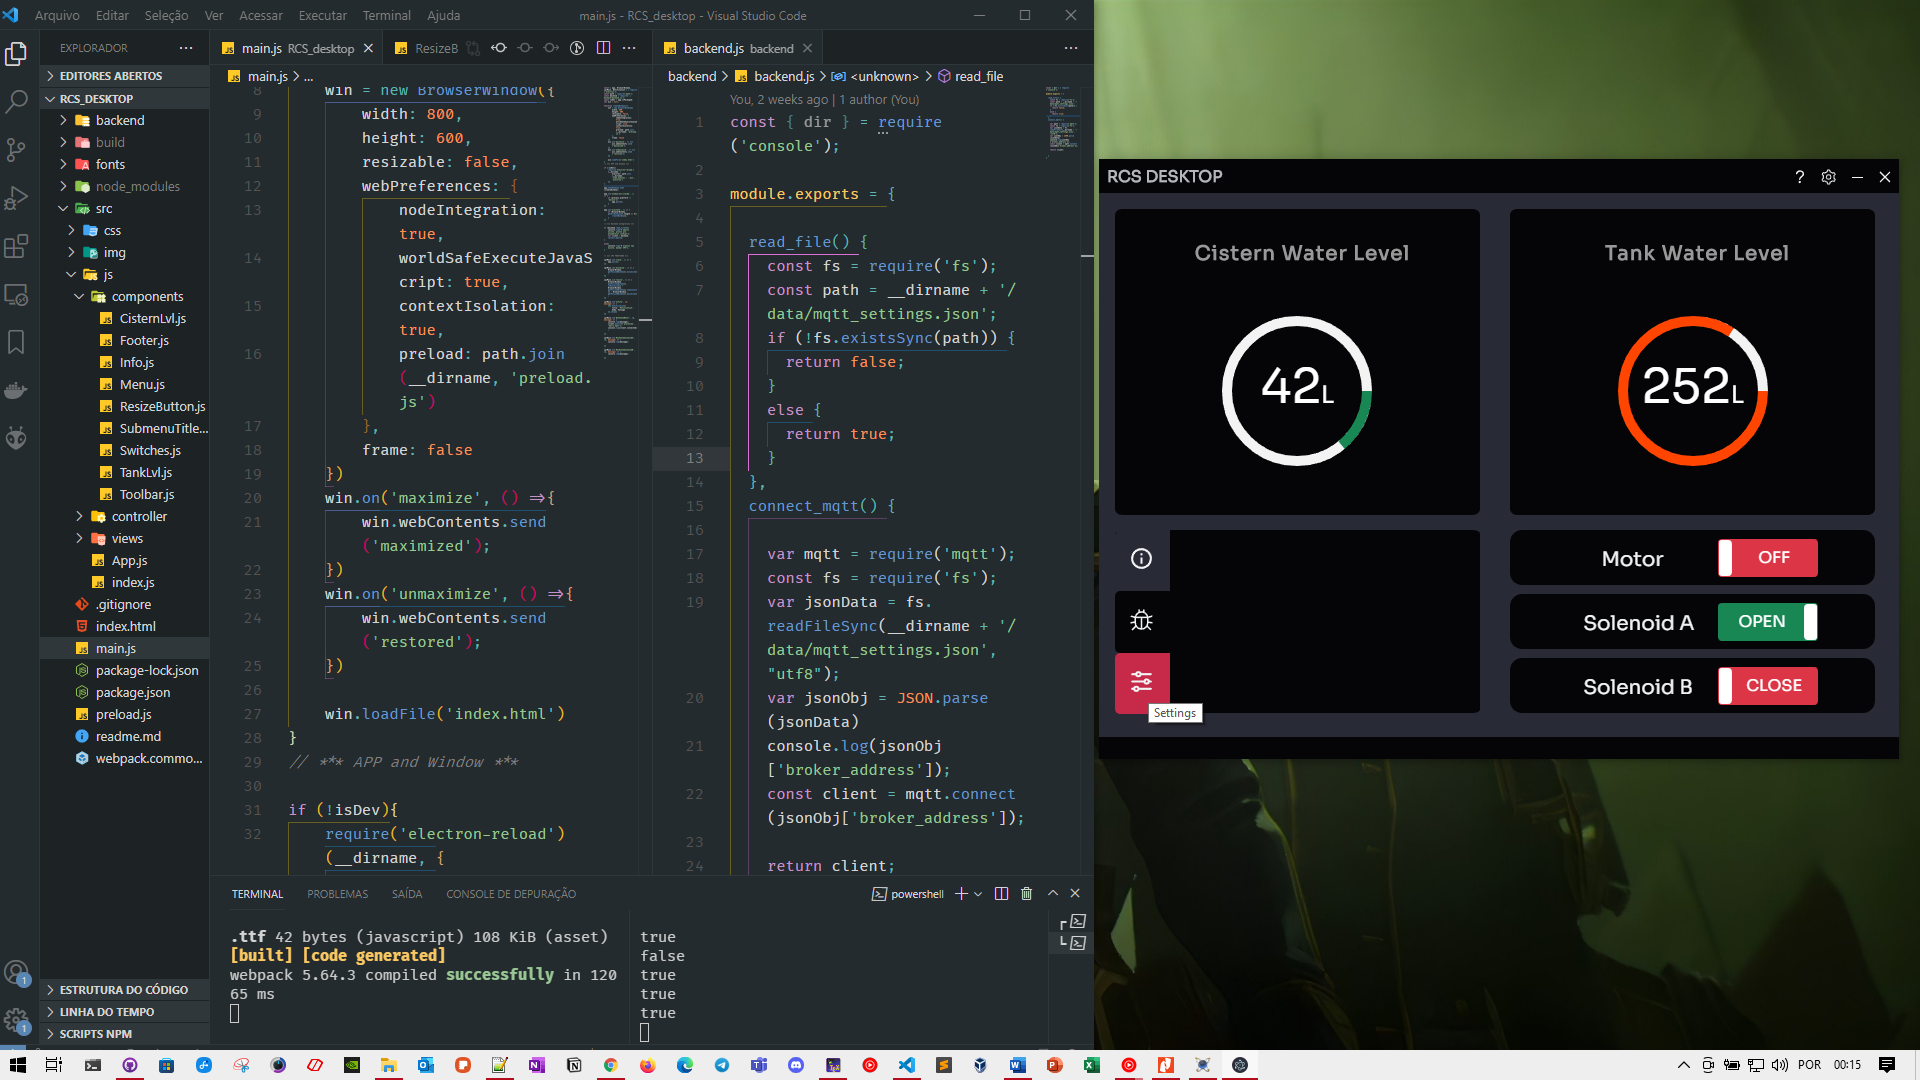
\includegraphics[width=1\textwidth]{figuras/rcs_desktop.png}
	\fonte{Própria}
	\label{fig:tela_desktop}
\end{figure}


\begin{figure}[H]
	\centering
	\caption{Implementação da aplicação \textit{mobile}.}
	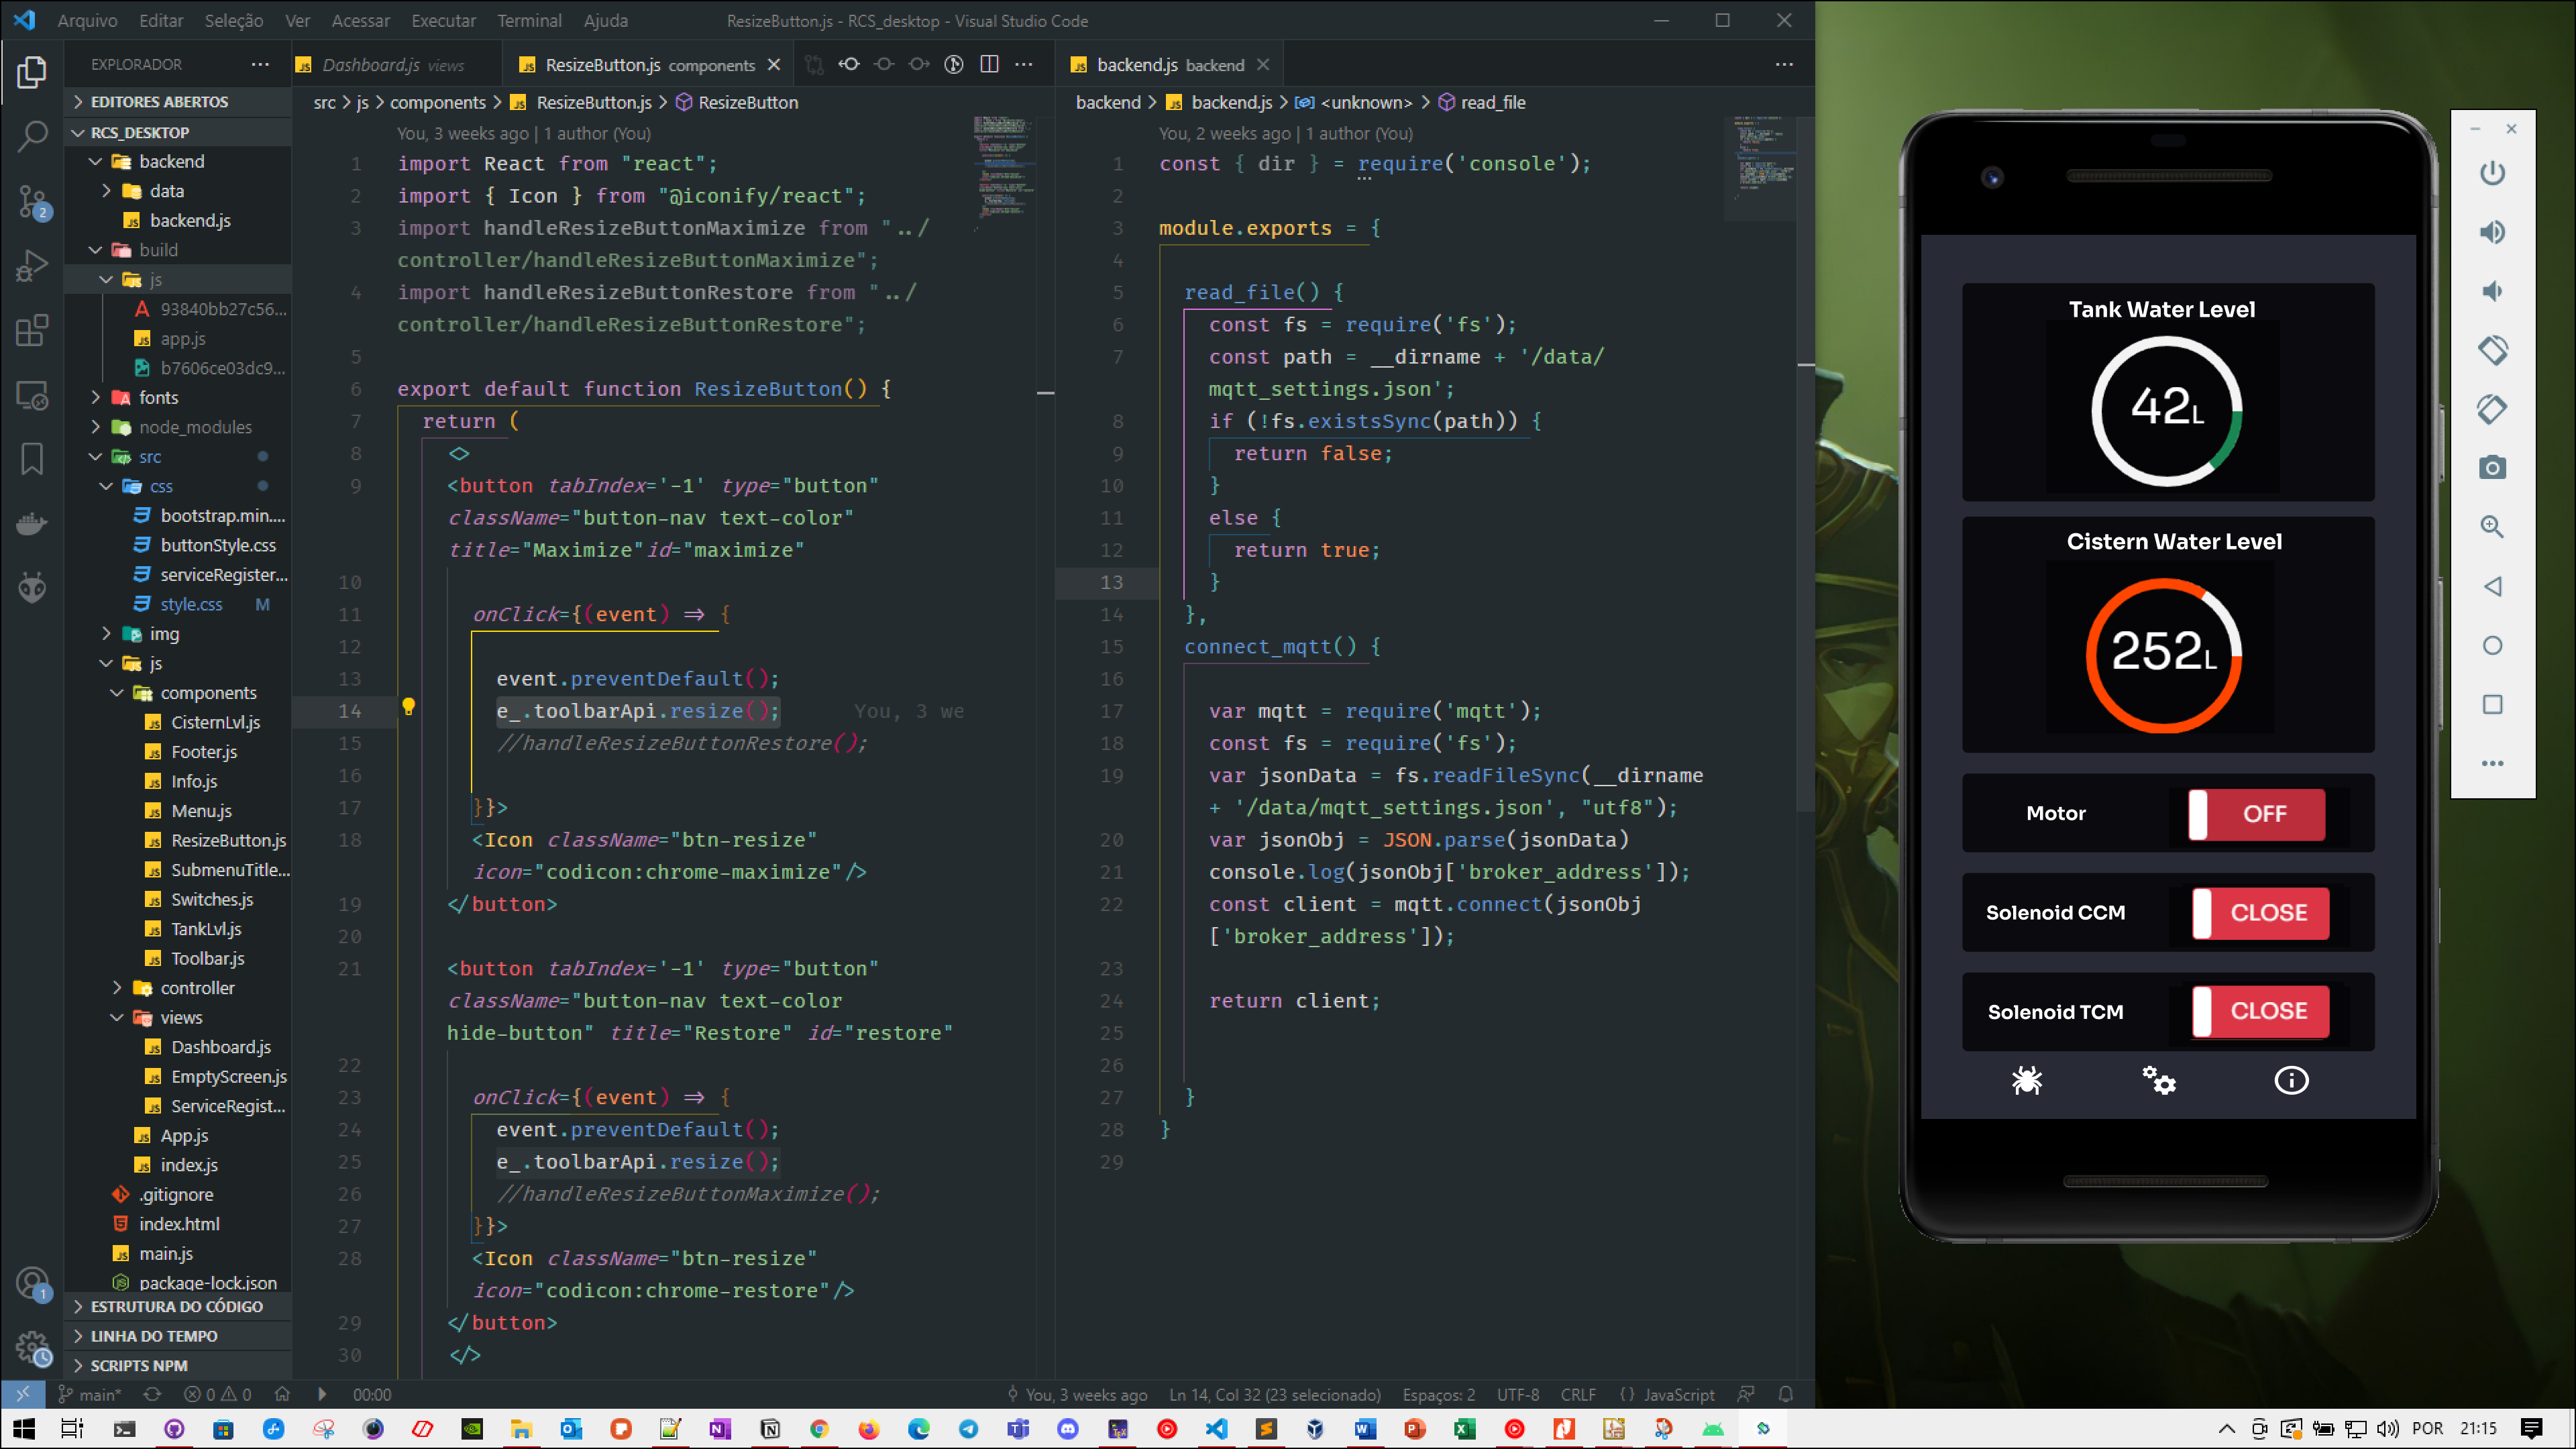
\includegraphics[width=1\textwidth]{figuras/rcs_mobile.png}
	\fonte{Própria}
	\label{fig:tela_mobile}
\end{figure}
